\section{Methodology} \label{sec:meth}

This section describes our evalauation methodology for evaluating proximate and running the
proximate parallel programs.

\subsection{Workloads}
We first describe the workloads we have targetted and then the methodlogy to 
evlauate them. Since, proximate is aimed at high performance and throughput
for both regular and irreguaar workloads, we have considered both class of workloads
and their parallel implementations. 

\paragraph{Regular Worklaods}
Regular worklaods are generally the high-performance computing applications
which have following properties: i) regular streaming memory access patterns,
ii) Computationally intensive and iii) ample amount of data-level parallelism.
We consider deep learning neural networks kernels similar to Diannao accelerator engine~\cite{diannao}
and the convolution based image processing workloads from Convolution Engine~\cite{convolution_engine}.
Some other micro-benchmarks for functional evalaution considered are: Ocean, summation and reduction, 
but we don't consider in our performance evalaution. 


\paragraph{Irregular Worklaods}
Irregular workloads generally have i) irregular memory access patterns
with low ILP, ii) Ver small computations and iii) Data dependent control. 
For such workloads, we consider the graph based workloads like histogram, 
shortest path and breadth-first-search. 


\subsection{Simualation Methodology} 
For proximate multi-core riscv inorder core simualtion, 
we consider a multi-core simualtor called ZSim~\cite{sanchez2013zsim}, which is a
fast x86-65 simulator. It is based on dynamic binary translation and PIN~\cite{pin} model which natively 
runs the pthread instances of the kernel on the real hardware.  

\begin{figure}
  \begin{center}
    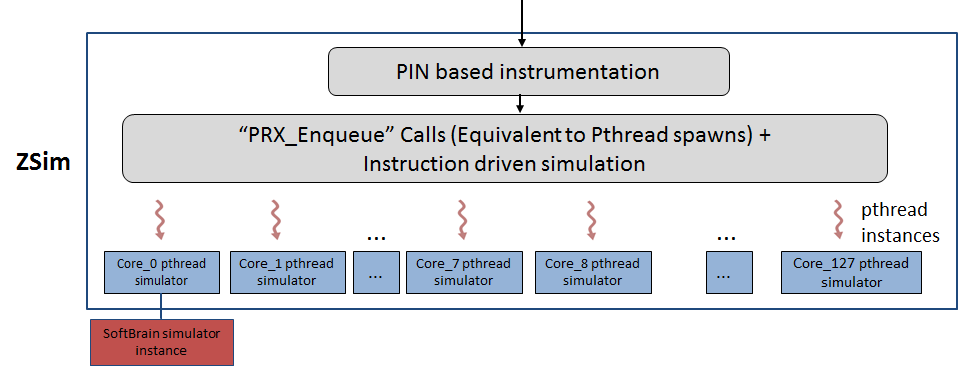
\includegraphics[width=\linewidth]{cs758-figs/zsim-meth.png}
  \end{center}
\vspace{-0.2in}
  \caption{ZSim based Proximate Simualtion}
  \label{fig:sim}
\vspace{-0.05in}
\end{figure}

Figure~\ref{fig:sim} shows our simulation methology, and  each compiled
proximate API based pthread program ins instrumented for multi-core simualtion initially.
Then, the proximate API based hooks would identify the proximate kernel and whenever ZSim main thread
encounters a \emph{PRX\_Enqueue} API call, it would offload the kernel to 
a) multiple in-order core pthread instances - if the kernel is an irregular type,  or b) Softbrain simualtor instance
which runs the softbrain portion of the kernel, if the kernel is a regualr type. 
Currenly, we don't have simualtor support to run, multiple instances of Softbrain kernels, 
and hence all the softbrain based parallel kernels need to be serialized to the same softbrain
simualtor instance. We aim to support this in our infrastructre in coming days. 


\begin{table}[]
  \centering
  \begin{tabular}{|l|l|}
    \hline
    \textbf{Baseline Configuiration} & \textbf{Explanation}                                \\ \hline
    \textit{pthread\_xeon}  & Pthread program run on a 64-core Xeon-Phi processor \\ \hline
    \textit{omp\_xeon}      & OpenMP program run on a 64-core Xeon-Phi processor  \\ \hline
  \end{tabular}
  \caption{Baseline Xeon-Phi configurations used for comaprison}
  \label{tab:base-config}
\end{table}

\subsection{Proximate Configurations}
In this section, we explain different configurations of proximate we have simulated, 
to compare agianst the real hardware. 

For comaprison of parallel program execution on proximate with
a server class processor, we first the baseline versions of parallel programs implemented in pthreads and OpenMP
running on r a 64-core 4way SMT Xeon-Phi processor.
Table~\ref{tab:base-config} explains the 2 baseline versions of parallel programs we run on Xeon-Phi machine.
We vary the number of threads for these 2 baselines, to find out the best design space w.r.t number of threads
and choose that as the comaprison point for proximate parallel program.

We now explain, the actual Proximate configurations simualted using the methodogy explained above. 
As we kno that current proximate hardware has \emph{1 host-core + 128 in-order cores + 1 Softbrain}, we try
to support the same hardware configuration in our simualtions. Although, ideally you would be needing 8 Softbrain 
instances runnign on each vault, our infrastrucure cannot support that for now and hence only 1 softbrain.

Based on kernel type, each proximate program can be simualted only on in-order cores without the quequing model
explained previoulsy here in Section~\ref{sec:queue}. Or, if more kernel instances are present in the program, then they 
can be dynamically spawned on the queuing model of proximate. When you have softbrain portions in the program, 
you would want to run on softbrain only simualtion. So, there are different ways of simuating proximate based on the kernel
type and Table~\ref{tab:real-configs} sumamrize the possible simaulted conifgurations for proximate. We would be using these
configurations for comparison in our evlaution. 


\begin{table}[]
  \centering
  \begin{tabular}{|l|l|}
    \hline
    \textbf{Proximate Configuration}               & \textbf{Explanation}                                                    \\ \hline
    \textit{prx\_inorder}                          & Proximate API pthread program w/o queuing model                         \\ \hline
    \textit{prx\_inorder\_q}                       & Proximate API pthread program with queuing model                        \\ \hline
    \textit{prx\_sb\_only}                         & Proximate API + single SoftBrain ‘only’ program                         \\ \hline
    {\color[HTML]{FE0000} \textit{prx\_multi\_sb}} & {\color[HTML]{FE0000} Proximate API + multi-threaded SoftBrain program -- Not simualted} \\ \hline
  \end{tabular}
  \caption{Proximate Simualted Configurations}
\label{tab"real-configs}
\end{table}
